\section{Durchführung}
\label{sec:Durchführung}

Der Versuch wird nach \autoref{fig:aufbau} aufgebaut. Eine Darstellung, wie der Aufbau in dem von uns durchgeführten Versuch aussah, ist in den Abbildungen \ref{fig:aufbau1} und \ref{fig:aufbau2} zu sehen.
\begin{figure}[H]
    \centering
    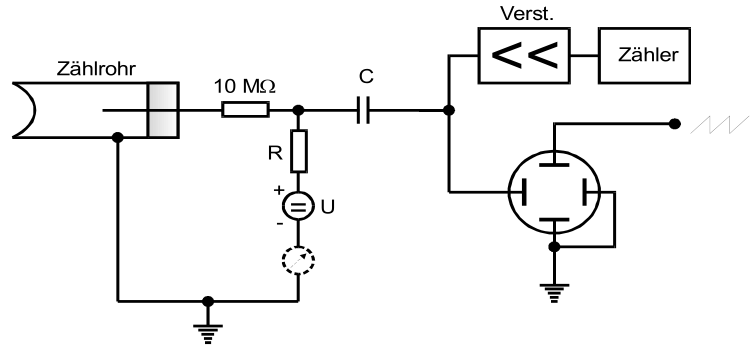
\includegraphics[width=0.75\textwidth]{data/Schaltplan.png}
    \caption{Schaltplan des Versuchaufbaus \cite{Anleitung703}.}
    \label{fig:aufbau}
\end{figure}

\begin{figure}[H]
    \centering
    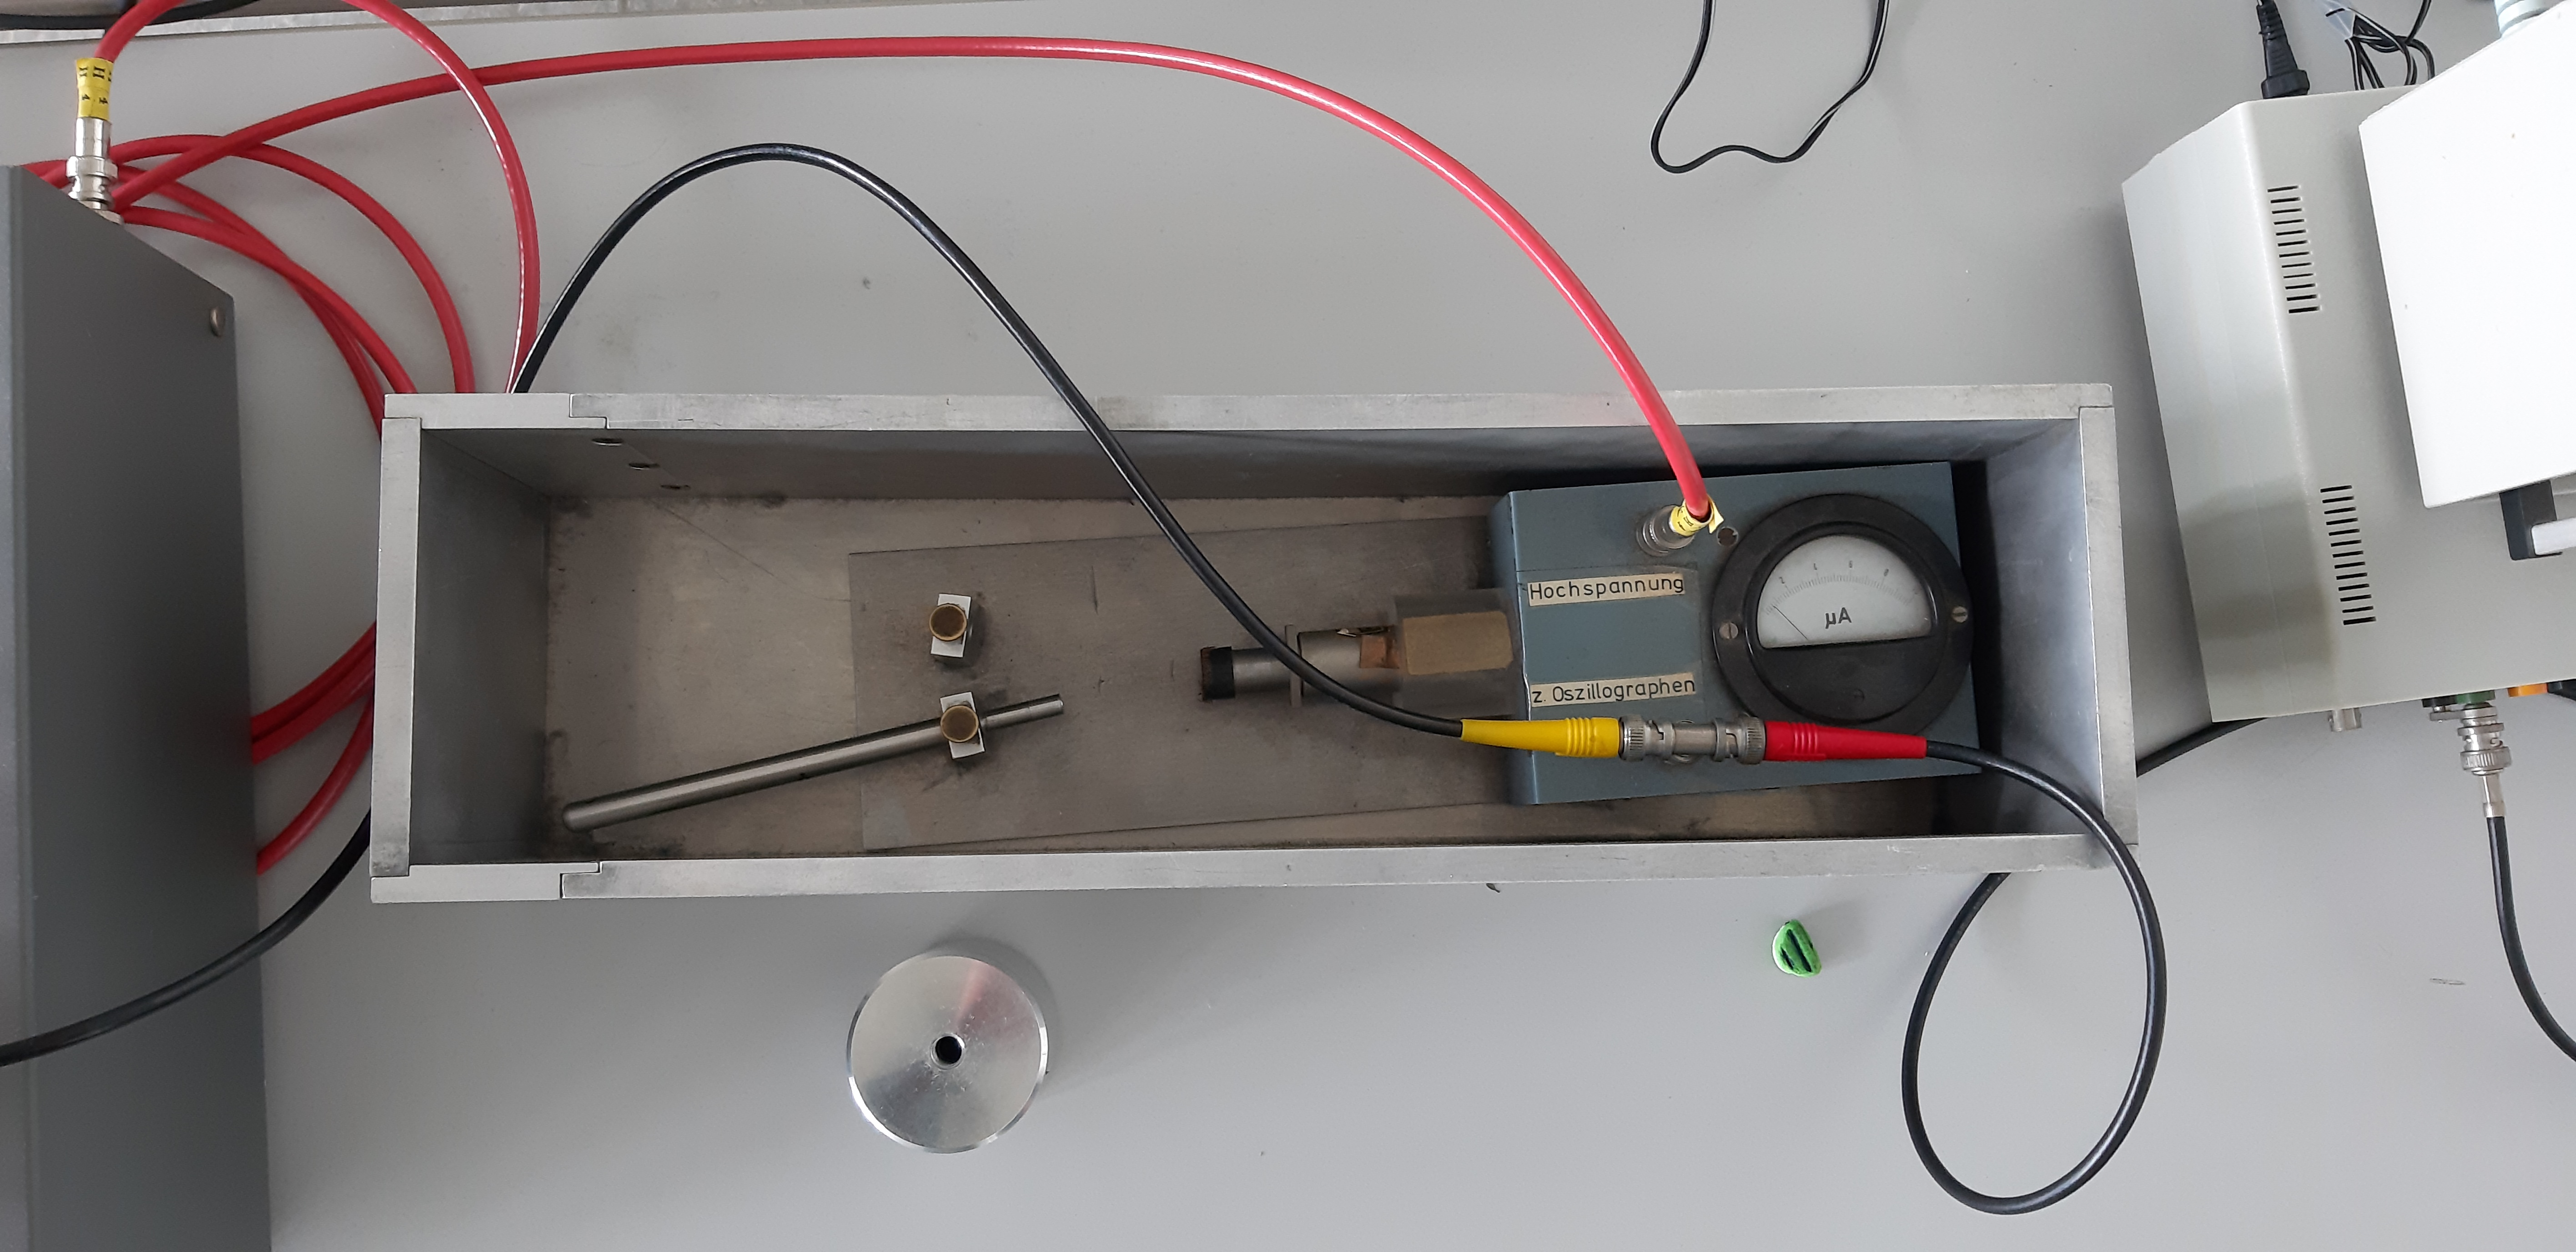
\includegraphics[width=0.75\textwidth]{data/kasten.jpg}
    \caption{Aufbau des Versuches.}
    \label{fig:aufbau1}
\end{figure}

\begin{figure}[H]
    \centering
    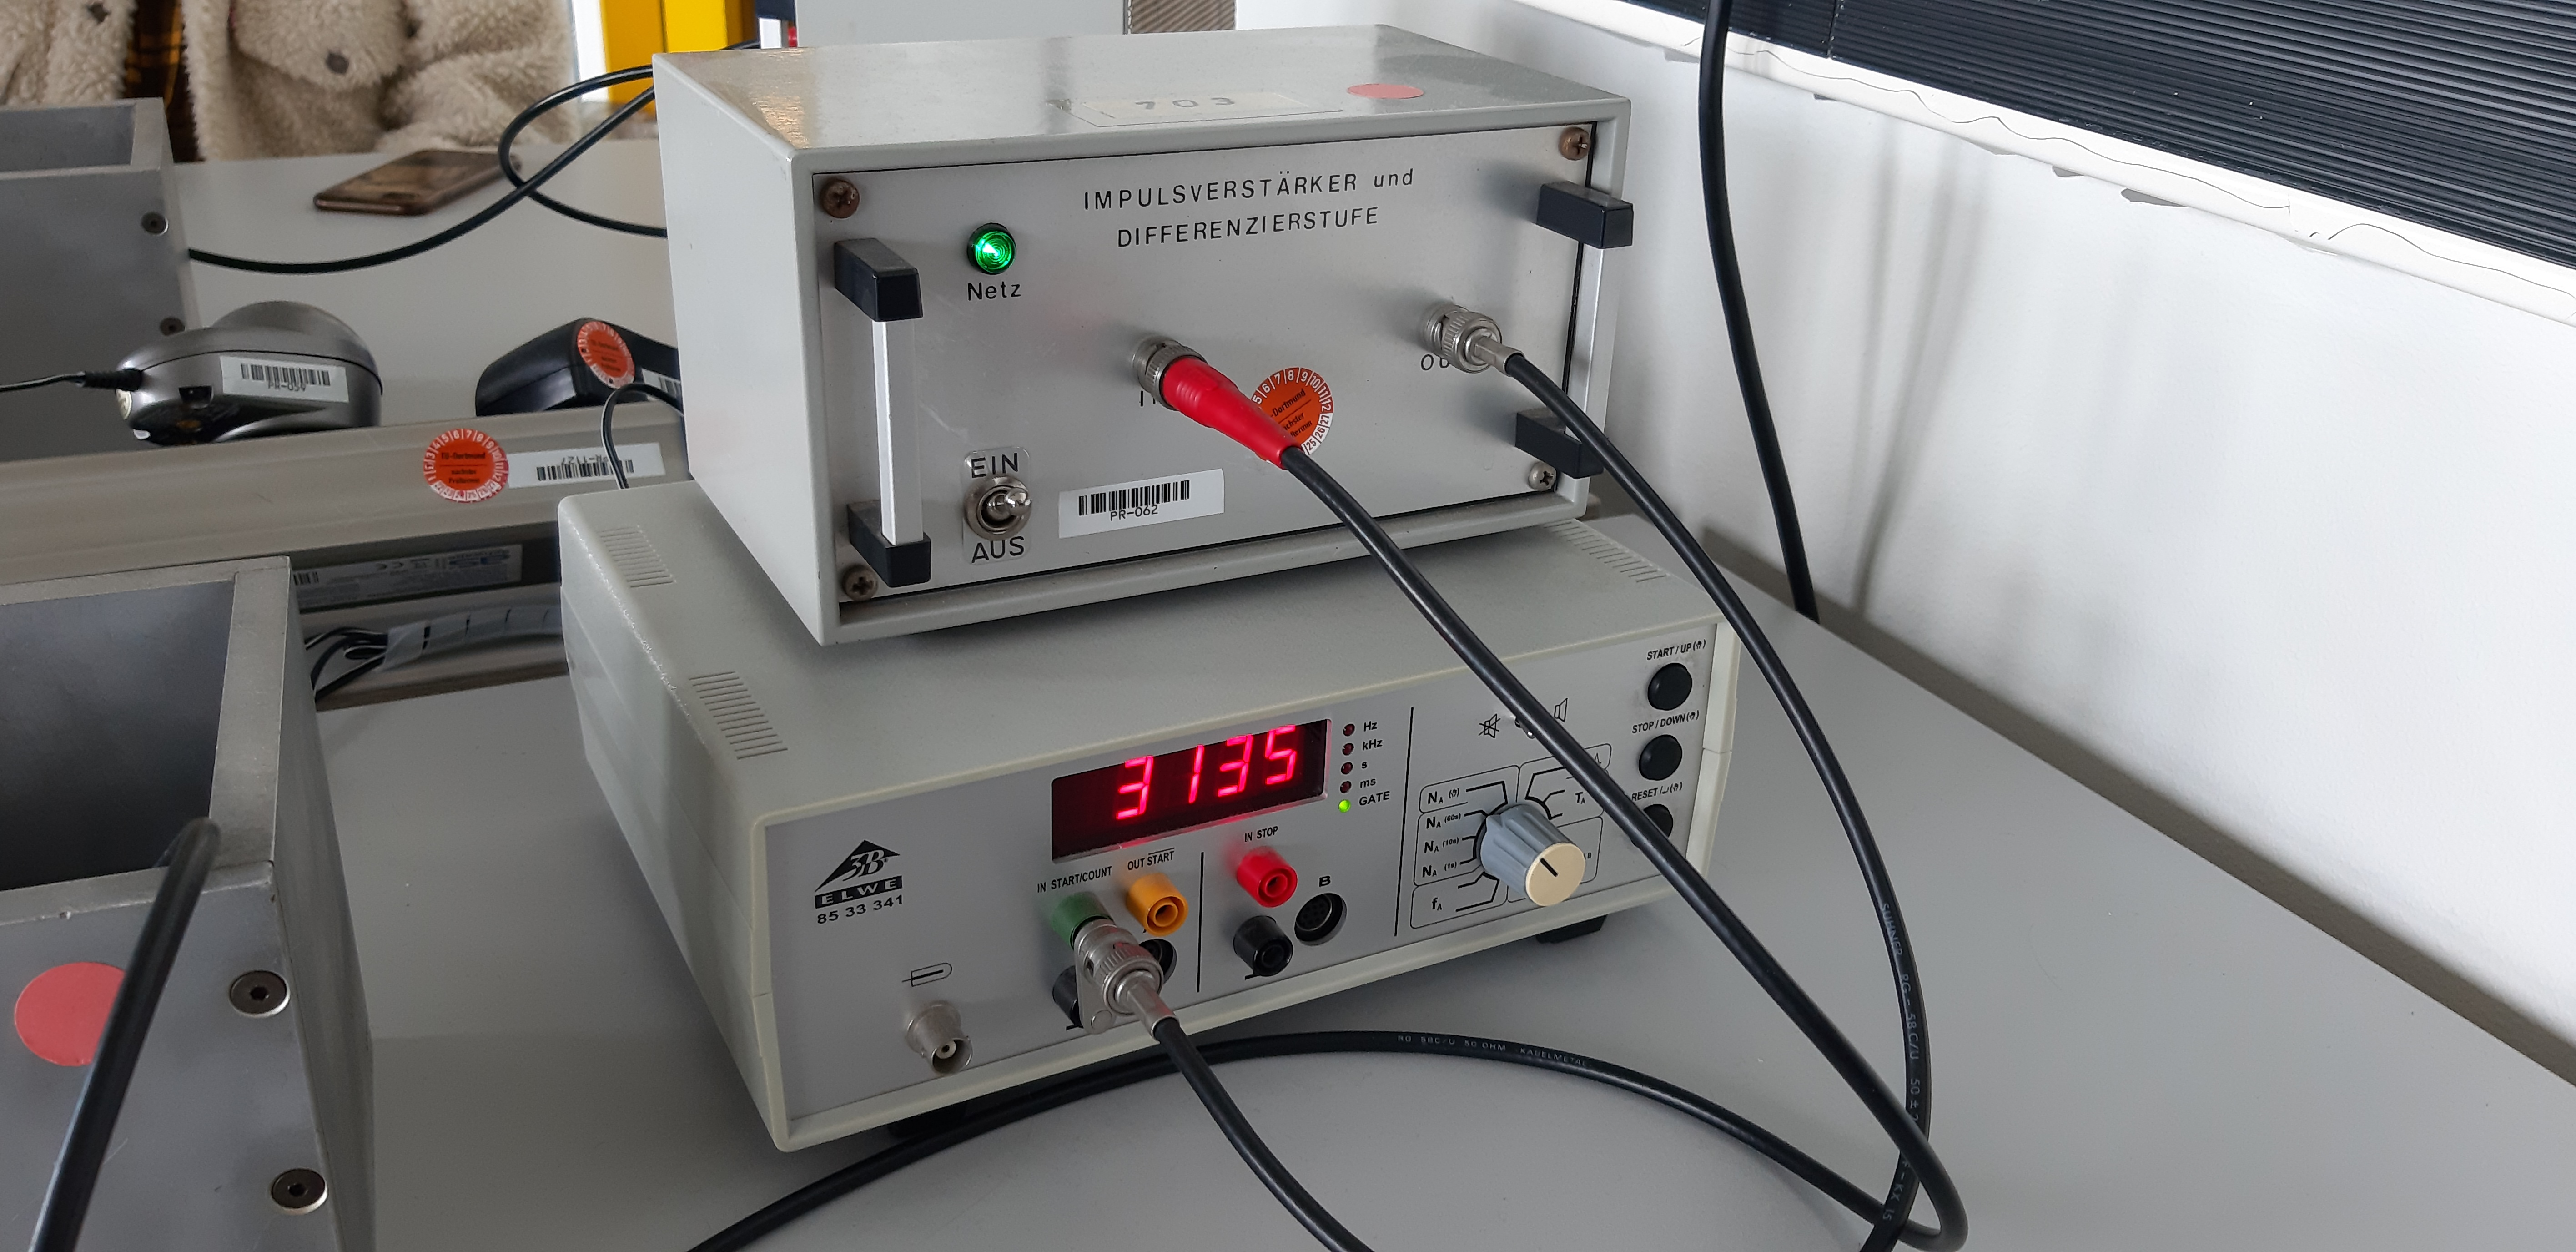
\includegraphics[width=0.75\textwidth]{data/geigerMueller.jpg}
    \caption{Aufbau der Messapparatur.}
    \label{fig:aufbau2}
\end{figure}

Im ersten Schritt wird ein $\beta$-Strahler vor das Fenster des Zählrohres positioniert. Es wird die Anzahl der in $\SI{120}{\second}$ einfallenden Elektronen in Abhängigkeit der Betriebsspannung $U$ in
einem Bereich von $\SIrange{300}{700}{\volt}$ gemessen. Dabei ist mit besonderer Vorsicht darauf zu achten, dass die Betriebsspannung die $\SI{700}{\volt}$ nicht übersteigt, da sonst der
Bereich der selbstständigen Gasentladung erreicht wird und das Zählrohr zerstört würde.
Während die einfallenden Elektronen gemessen werden, wird gleichzeitig der Zählrohrstrom gemessen werden. \newline
In einem zweiten Schritt wird mithilfe des Ozilloskopes die Plateausteigung qualitativ untersucht. Die Strahlungsintensität der $\beta$-Quelle wird dabei soweit herabgesetzt, dass kein weiterer Impuls eines 
$\beta$-Teilchens auf dem Bildschirm zu sehen ist. Außerdem muss die Betriebsspannung auf etwa $\SI{350}{\volt}$ herabgesetzt werden, sodass die Nachentladungen vernachlässigbar gering sind.
Mithilfe der aufgenommenen Daten wird auch die Totzeit gemessen. \newline
Im letzten Schritt wird mithilfe der Zwei-Quellen-Methode erneut die Totzeit bestimmt. Dazu wird zuerst die Zählrate eines einzelnen Präparates gemessen. Danach wird ein zweites hinzugefügt, ohne das die Lage des ersten relativ zum Zählrohr verändert wird.
Es wird erneut die Zählrate der eintreffenden Teilchenanzahl mit beiden Quellen gemessen. Als letztes wird das erste Präparat entfernt und nur die Zählrate des zweiten gemessen.